% !TEX root = ../thesis.tex

\vspace{-10pt}

\section{User Interface Design}

\vspace{-10pt}

Lyra was developed through an iterative user-centered design process. We held
formative interviews with representative users, such as visualization designers
and journalists, to understand their design process and the limitations of their
existing tools. These users evaluated low-fidelity prototypes and later
interactive prototypes.

The Lyra interface, as shown in \cref{fig:lyra:teaser}, is split into three
sections. The left-hand panel (\cref{fig:lyra:inspectors}(a)) depicts \emph{data
pipelines}: chains of data transformations applied to a data source. A
pipeline's inspector provides a paginated data table showing the output of the
pipeline, buttons to add new transformations, and a list of scales defined over
data fields. The right-hand panel (\cref{fig:lyra:inspectors}(c)) contains
inspectors for graphical elements such as marks, axes, and legends. These
elements are grouped into \emph{layers} to determine coordinate spaces and
z-ordering. These inspectors list all visual properties (position, fill color,
angle, etc.) along with widgets to manipulate them. The central panel contains
the visualization canvas where graphical elements may be directly manipulated.

\begin{figure}[t!]
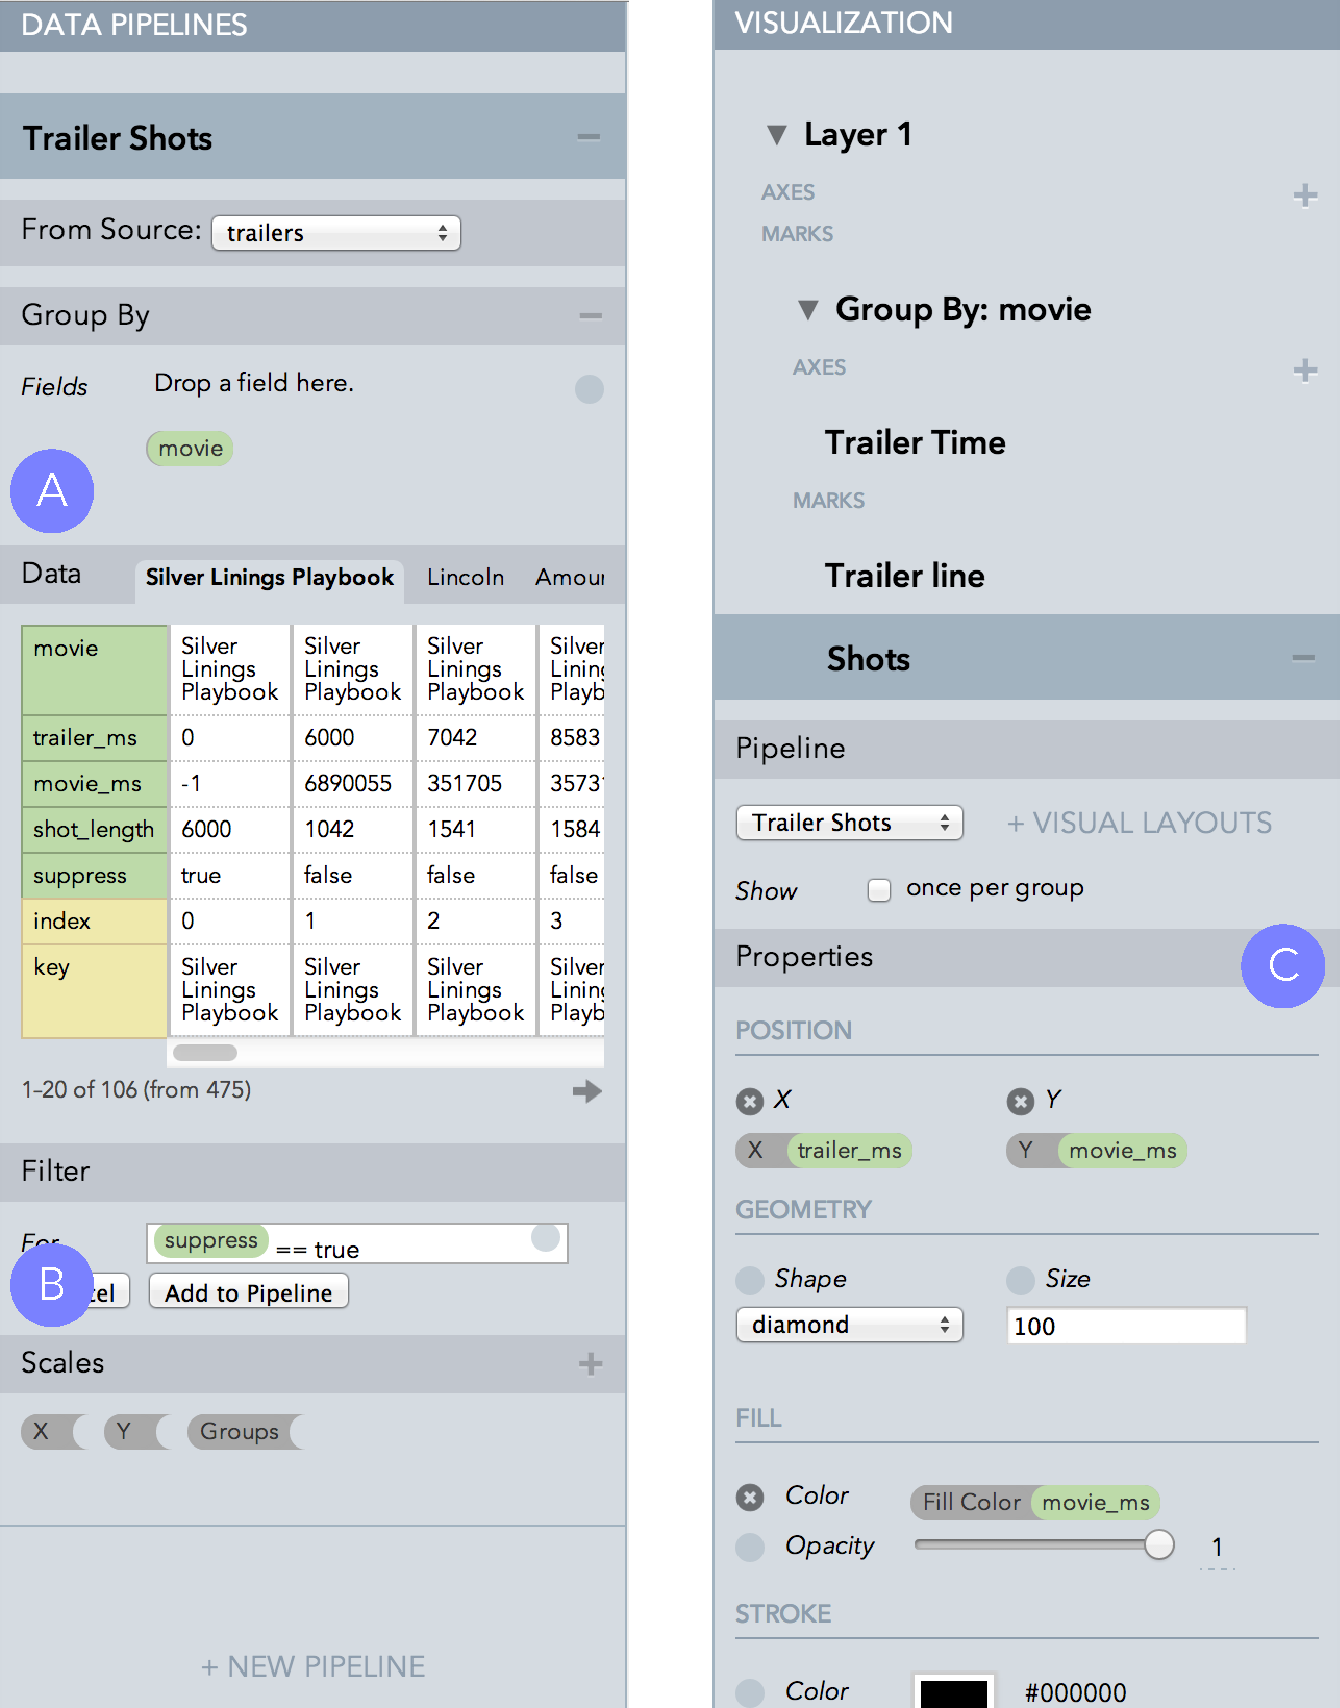
\includegraphics[width=0.9\columnwidth]{inspectors}
\caption{Lyra's side panels for data pipelines (left), and
visual properties (right). (a) Data table showing the current output
of the pipeline; (b) Scale transforms defined over fields in the pipeline.
(c) A property inspector for a symbol mark type; two properties have been
mapped to data fields.}
\label{fig:lyra:inspectors}
\end{figure}

\vspace{-10pt}

\subsection{Data Pipelines}

\vspace{-7pt}

Lyra's left-hand panel contains \emph{data pipelines}: workflows of transforms
applied to input data. Clicking a pipeline reveals an inspector that lists
applicable transforms and presents a paginated table view of transformed data.

\textbf{Data Table View}. Data pipelines include a data table view, using a
layout inspired by Bret Victor~\cite{victor:drawing}. The first column in the
table view lists field names, enabling vertical scanning. Subsequent columns
display individual records (\cref{fig:lyra:inspectors}(a)). Field names in the
first column are interactive: clicking a field sorts the table by that
dimension, drag-and-drop can be used to bind fields to mark properties. Fields
are colored by their source: green for fields in the original data and yellow
for fields derived by a transform. For example, the \emph{formula} transforms
adds new fields based on mathematical expressions. When \emph{group by}
transforms are applied, one tab for each group appears above the table view.

\textbf{Authoring Transforms}. Users can add a transform by clicking the
corresponding icon and configuring its parameters. Users may preview the effect
of applying a transformation in a popover. Once a transformation is added to the
pipeline, adjusting its properties is reflected in real-time across the table
view and the visualization.

\textbf{Scales}. The inspector also lists all scales defined over data fields in
the pipeline (\cref{fig:lyra:inspectors}(b)). Lyra automatically instantiates
scales when a field is associated with a mark property. The scale domain is
defined over the field values; the range is determined using production rules
described below. Users can also create scales manually. Users can drag scales
onto mark properties to apply a scale transform, or click a scale to access an
editor dialog (see \cref{fig:lyra:usage}(e)). When editing a scale that is not
represented by an axis or legend, a transient guide is shown in the canvas to
convey the effect of scale changes.

\vspace{-10pt}

\subsubsection{Design Rationale}

\vspace{-10pt}

Our initial prototypes hid raw data values in favor of exposing only the table
schema. However, evaluations indicated this was insufficient. Users noted that
it was difficult to determine the effect of a data transformation based solely
on the visualization. Moreover, the incremental nature of visualization design
can lead to unexpected intermediate output, for example setting the
\texttt{height} of a rectangle mark can cause all mark instances to overlap if
no \texttt{x} or \texttt{width} property has been set. Later prototypes
introduced a full data table view, to enable inspection of raw values and expose
the current data organization.

Similarly, early prototypes masked the presence of scales: mapping data to
visual properties automatically instantiated a scale, but they were not
explicitly exposed in the interface. When users attempted to construct
visualizations, we found that this significantly restricted their
expressiveness. For example, it is often necessary to specify custom ranges
for scales rather than rely on preset ranges. Such modification is difficult
to do without surfacing scales as a first-class construct. Later evaluations
found that users additionally had trouble identifying the purpose of scales,
or the effects of scale modification, if the scales were not explicitly
represented on the visualization by an axis or legend guide. In response, we
introduced transient guides.

\vspace{-10pt}

\subsection{Composing Visual Elements}

\vspace{-7pt}

Visualizations in Lyra are compositions of visual elements: graphical
\emph{marks} and \emph{guides}. Elements are grouped together into
\emph{layers}, which define local coordinates and establish z-ordering. Lyra's
right-hand panel lists the layers and their elements
(\cref{fig:lyra:inspectors}(c)). Elements are added to a visualization by
creating them within this panel or by dragging a mark from the mark palette.
When an element is selected, an inspector presents all the element's associated
properties. Property values may be edited directly or set via drag-and-drop of
data fields with changes reflected on the visualization in real-time. Hovering
over a property displays a guide overlaid on the visualization to illustrate how
that particular property affects the rendered output. Visual elements can also
be manipulated directly on the visualization canvas.

\begin{wrapfigure}{l}{0pt}
  \raisebox{0pt}[\dimexpr\height-0.85\baselineskip\relax]{
\includegraphics
  [width=0.6cm]{handles}}
\end{wrapfigure}

\vspace{5pt}
\noindent
\textbf{Handles} in the canvas can be used to interactively move, rotate and
resize selected elements. A mark definition will typically render one mark
instance per datum in the visualization. To reduce visual clutter, selecting a
mark displays handles only on the instance that was clicked. However, when a
user adjusts the handles, the change is reflected simultaneously across all mark
instances.

\begin{wrapfigure}{l}{0pt}
  \hspace{-12pt}
  \raisebox{0pt}[\dimexpr\height-0.9\baselineskip\relax]{
  
\includegraphics
  [width=1cm]{connectors}}
\end{wrapfigure}

\vspace{5pt}
\noindent
\textbf{Connectors} can be used to position marks relative to one-another.
Dragging a target mark onto a host mark's connector establishes a connection:
the target mark's position is now determined by the host's properties. Changes
to the host mark automatically propagate to all connected targets. Connectors
are particularly useful for positioning text labels relative to other marks.

\begin{wrapfigure}{l}{0pt}
  \raisebox{0pt}[\dimexpr\height-0\baselineskip\relax]{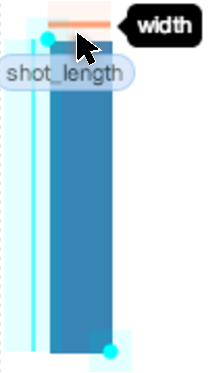
\includegraphics
  [width=1.8cm]{dropzones}}
\end{wrapfigure}

\vspace{5pt}
\noindent
\textbf{Drop zones} are used to associate data fields with mark properties. When
dragging a data field, drop zones overlay the visualization canvas. Each drop
zone comprises a shaded region and a guide line or point to indicate the
corresponding mark property (e.g., \texttt{x}, \texttt{width}, etc.). Hovering
on a drop zone highlights it and shows the property name in a tooltip. Dropping
a field then establishes a mapping between the data field and the mark property.
To avoid clutter, Lyra shows drop zones only for the currently selected item.
When dragging a data field, users can hover and pause over a mark instance to
make it the selected item.

\vspace{-10pt}

\subsubsection{Design Rationale}

\vspace{-10pt}

Surfacing all properties in the inspector was an immediate first step to ensure
that Lyra maintained Vega's expressivity. Users noted that these inspectors were
akin to Tableau's ``shelves,'' a familiar interaction paradigm for many of them.
However, there remained a clear opportunity to further narrow the gulf of
execution~\cite{hutchins:directmanip} by pushing interactions to the
visualization canvas itself. For example, we observed users attempting to
select, move, or resize marks currently visualized on the canvas.

As users cited familiarity with drawing tools, we sought to reuse familiar
interaction mechanisms with \emph{handles} and \emph{connectors}. However, there
is not a similarly established interaction mechanism for data-property bindings.
We ultimately arrived at our \emph{drop zones} design by prototyping a number of
alternatives. One such alternative incorporated flow
menus~\cite{guimbretiere:flowmenu}. When dragging a data field over a mark on
the canvas, a flow menu would appear listing all mappable visual properties.
When dragging the field over a property, a submenu would appear listing
appropriate scale types given the type of the data field, and the particular
property. For example, for fields with numeric data, this submenu offered all
quantitative scale types including linear, logarithmic, and so forth. Dropping
the field over a particular scale type established a mapping and instantiated
the appropriate scale.

In addition to testing designs with users, we analyzed them using the Cognitive
Dimensions of Notation heuristics~\cite{blackwell:cogdim}. Data mapping through
flow menus, for example, provided a \emph{visible} and \emph{consistent}
interface---regardless of the mark type, all properties were consistently
ordered within the top-level menu. Although exposing scale types in the submenu
arguably reduced \emph{error\--proneness} (as Lyra need not infer a scale type),
it increased the \emph{diffuseness} (or verbosity) of the interface. User
feedback also revealed that selecting an option from this submenu was a
\emph{hard mental operation} as it forced them to select a particular scale type
up front. Many users perceived this as a \emph{premature commitment}. Perhaps
most troublesome, given our goal of reducing the gulf of execution, was the lack
of a \emph{closeness of mapping}: properties were listed as menu items, one
after another.

Drop zones, on the other hand, achieve a high \emph{closeness of mapping} as
they overlay the canvas in a way that corresponds to the property they
represent. For example, a rectangle's \texttt{x2} drop zone is shown extending
from the left edge of the canvas to the right-most edge of the rectangle.
Dropping a field over a drop zone performs \emph{scale inference} (described
below) to reuse an existing scale definition or instantiate a new one. Although
this may increase \emph{error-proneness}, it decreases \emph{diffuseness} and
reduces the \emph{hard mental operations} flow menus presented. One limitation
of drop zones is a subtle lack of \emph{consistency}; for example, a tall
rectangle mark will present a larger \texttt{height} drop zone than a shorter
one. We mitigate this issue by showing drop zones only for the currently
selected mark.

\vspace{-10pt}

\subsection{Scale Inference and Production Rules}

\vspace{-7pt}

When a user binds a data field to a mark property, Lyra performs \emph{scale
inference} in an attempt to reuse existing scale definitions. Lyra searches for
an existing scale with the field as its domain. If a scale is found, it is
reused if its range type is appropriate (e.g., spatial or color values). If no
scale is found or the range type does not match, Lyra instantiates a new scale:
ordinal for categorical data or linear for quantitative data, along with a
default range based on the property type (e.g. \texttt{width} for \texttt{x}
properties).

To accelerate common encoding decisions, Lyra also uses a set of context- and
mark-specific \emph{production rules} to determine intelligent defaults. These
production rules may set additional properties of the mark or add new graphical
elements to the canvas. For example, dropping a field over a rectangle mark's
\texttt{width} drop zone automatically binds the \texttt{x} property as well to
correctly position each rectangle. Dropping a field over a spatial property may
add an axis; dropping a field over a color property may add a legend. A user can
customize these defaults using the property inspector. However, users may
occasionally wish to sidestep the production rules. Accordingly, Lyra evaluates
production rules only when a mapping is established using drop zones. If the
user instead drops a data field onto the property inspector panel, no production
rules are evaluated and so no defaults are added.

\vspace{-10pt}

\subsubsection{Design Rationale}

\vspace{-10pt}

Scale inference and production rules were informed primarily by early user
feedback. Without these features, users had to manually create every aspect of
the visualization, which they found to be tedious. Users did not expect to have
to specify a scale definition on every data mapping operation, and expected axes
or legends to be automatically added as appropriate. We found that the features
did alleviate this tedium but, interestingly, users subsequently requested a
method of circumventing them \emph{``if they knew better''}. As a result,
although Lyra performs scale inference on every data field mapping, production
rules are only evaluated if the data field is dropped over a drop zone. Users
may sidestep the rules by working directly with property inspector instead. We
fully enumerate Lyra's scale inference procedure and production rules in
supplementary material.

\vspace{-10pt}

\subsection{Saving and Exporting Visualizations}

\vspace{-7pt}

Visualizations built in Lyra can be exported as static \textsc{png} or
\textsc{svg} files, or as Vega \textsc{json} specifications. With Vega's
JavaScript runtime, the \textsc{json} file can be parsed and rendered on a web
page, dynamically bound to new input data, and extended with interactions.